\documentclass[12pt,a4paper]{article}
\usepackage[utf8]{inputenc}
\usepackage[T1]{fontenc}
\usepackage{amsmath,amssymb}
\usepackage{pgfplots}
\usepackage{tikz}
\usepackage{lmodern}
\usepackage{graphicx}
\usepackage{hyperref}
\usepackage{listings}
\usepackage{xcolor}
\usepackage{enumitem}
\usepackage{fancyhdr}
\usepackage{lastpage}
\usepackage[left=2.5cm,right=2.5cm,top=2.5cm,bottom=2.5cm]{geometry}
\usepackage[table]{xcolor}
\usepackage{array}
\usepackage{hyperref}
\usepackage{nameref}

\pagestyle{fancy}
\fancyhf{}
\renewcommand{\headrulewidth}{0pt}
\rfoot{\thepage\ af \pageref{LastPage}}

\title{Forløbsplan}
\author{Anders S. Østergaard}
\date{\today}

\definecolor{codegreen}{rgb}{0,0.6,0}
\definecolor{codegray}{rgb}{0.5,0.5,0.5}
\definecolor{codepurple}{rgb}{0.58,0,0.82}
\definecolor{backcolour}{rgb}{0.95,0.95,0.92}
\definecolor{darkerlightblue}{rgb}{0.1, 0.3, 0.5}

\lstdefinestyle{mystyle}{
	backgroundcolor=\color{backcolour},   
	commentstyle=\color{codegreen},
	keywordstyle=\color{darkerlightblue},
	numberstyle=\tiny\color{codegray},
	stringstyle=\color{codepurple},
	basicstyle=\ttfamily\footnotesize,
	breakatwhitespace=false,         
	breaklines=true,                 
	captionpos=b,                    
	keepspaces=true,                 
	numbers=left,                    
	numbersep=5pt,                  
	showspaces=false,                
	showstringspaces=false,
	showtabs=false,                  
	tabsize=2
}
\lstset{style=mystyle}
\usepackage{matlab-prettifier}
\begin{document}
	\begin{titlepage}
	\centering
	\vspace*{6cm}
	{\Huge\bfseries SWROB2\par Exam\par}
	\vspace{2cm}
	Submitted by: \par 
	\begin{table}[!h]
		\centering
		\begin{tabular}{|l|l|l|}
			\hline
			Study nr  & Name 					   & Study line\\\hline
			202005180 & Nicolaj Meldgaard Pedersen & E\\\hline
			202105443 & Johannes Baagøe 		   & E\\\hline
			201270449 & Anders Sandø Østergaard    & EP\\\hline
			201905293 & Daniel F. Borch Olsen	   & E\\\hline
		\end{tabular}
	\end{table}
	\vspace{4cm}
	Århus Universitet \par
	\vfill
	\today
\end{titlepage}
\pagenumbering{arabic}
\thispagestyle{empty}
\begin{abstract}
	\textit{This report presents the design, implementation, and evaluation of an advanced robotic system integrated with the Robot Operating System (ROS). The project leverages ROS's dynamic capabilities alongside sophisticated algorithms to enhance robotic functionalities in motion control, motion planning, perception using camera algorithms, localization, and mapping. Utilizing MATLAB and a specific hardware setup, the system demonstrates significant improvements in task efficiency and obstacle management within a controlled experimental setup. The findings highlight the system’s robustness in real-time operations and its potential for adaptation in varied automation scenarios. This study not only showcases the successful application of ROS in complex robotic tasks but also sets a foundation for future advancements in robotic automation. The report concludes with an analysis of experimental results, discussing the system's performance against predefined objectives and suggesting areas for further research.}
\end{abstract}
\clearpage
\tableofcontents
\clearpage

	\clearpage
	\section{Purpose}
	This document serves as a comprehensive guide aimed at facilitating the setup of a simulation environment for the TurtleBot 3. It is intended for students, researchers, and robotics enthusiasts who wish to explore the capabilities of TurtleBot 3 within a simulated environment before implementing solutions in real-world scenarios. By following the steps outlined in this guide, readers will be able to install and configure the necessary software components, including ROS Noetic, Gazebo, and the TurtleBot 3 packages, on a Ubuntu 20.04 LTS system.
	\\\\
	The simulation environment provides a safe and cost-effective platform for testing algorithms, developing robotics applications, and conducting experiments without the need for physical hardware. It offers an accessible entry point into the world of robotics, emphasizing hands-on learning and experimentation. Through this guide, we aim to empower users with the knowledge to successfully establish a robust simulation setup, enabling them to simulate a variety of tasks and scenarios with the TurtleBot 3.
	\\\\
	Additionally, this guide underscores the importance of understanding the underlying principles of robot operation, ROS architecture, and simulation dynamics. By the end of this setup, users will be well-equipped to navigate the ROS ecosystem, leverage the TurtleBot 3's features, and extend their exploration to more advanced robotics concepts and applications.
	
	\section{System Requirements and Compatibility}
	The choice of operating system is crucial for a seamless installation and operation of ROS (Robot Operating System). ROS Noetic Ninjemys, being the thirteenth release of ROS, officially supports Ubuntu 20.04 LTS (Focal Fossa). This compatibility is designed to leverage the long-term support and stability offered by Ubuntu 20.04 LTS, ensuring that developers have access to consistent updates and security patches. 
	\\\\
	It is highly recommended to use Ubuntu 20.04 (Focal Fossa) LTS as the primary operating system for installing ROS Noetic to avoid potential compatibility issues that may arise with other versions of Ubuntu or different Linux distributions. Ubuntu 20.04 LTS provides an optimal foundation for running ROS Noetic, thanks to its updated libraries, improved security features, and enhanced performance. 
	\\\\
	While ROS Noetic might be installed on newer versions of Ubuntu or through the use of Docker containers on other operating systems, such setups may require additional configuration steps and might not provide the same level of stability and support as the recommended Ubuntu 20.04 LTS platform. Users opting for alternative methods should be prepared for a more complex installation process and potential troubleshooting.
	\\\\
	Ensuring the alignment between the operating system and ROS version is essential for developers and researchers aiming to utilize the full spectrum of ROS features and capabilities without encountering unnecessary obstacles. By adhering to the recommended system requirements, users can expect a smoother installation experience and more reliable system performance during their robotics development and simulation endeavors.
	
	\section{VMware Installation}
	\begin{enumerate}
		\item Visit the official VMware website and download either VMware Workstation Pro or \href{https://www.vmware.com/products/workstation-player.html}{VMware Player}.
		\item Follow the on-screen instructions to install VMware on your host machine.
	\end{enumerate}
	
	\section{Ubuntu 20.04 LTS Installation in VMware}
	\begin{enumerate}
		\item Launch VMware and select "Create a New Virtual Machine".
		\item Choose "Installer disc image file (iso)" and browse to select your downloaded \href{https://releases.ubuntu.com/focal/}{Ubuntu 20.04 LTS ISO file}.
		\item Complete the guided setup, allocating desired resources (disk space, memory, CPU).
		\item Proceed with the Ubuntu installation process within the VM, creating a user account when prompted.
	\end{enumerate}
	
	\section{ROS Noetic Installation}
	Follow this tutorial or visit \href{https://wiki.ros.org/noetic/Installation/Ubuntu}{This Link}.\\
	Open a terminal in Ubuntu (no specific directory required).
	\begin{enumerate}
		\item Add the ROS Noetic repository:
		\begin{verbatim}
			sudo sh -c 'echo "deb http://packages.ros.org/ros/ubuntu 
			$(lsb_release -sc) main" > /etc/apt/sources.list.d/ros-latest.list'
		\end{verbatim}
		
		\item Install curl and add the ROS key:
		\begin{verbatim}
			sudo apt install curl
			curl -s https://raw.githubusercontent.com/ros/rosdistro/master/ros.asc | 
			sudo apt-key add -
		\end{verbatim}
		
		\item Update apt sources and install ROS Noetic Full Desktop:
		\begin{verbatim}
			sudo apt update
			sudo apt install ros-noetic-desktop-full
		\end{verbatim}
		
		\item Add ROS environment setup to your bash session:
		\begin{verbatim}
			echo "source /opt/ros/noetic/setup.bash" >> ~/.bashrc
			source ~/.bashrc
		\end{verbatim}
	\end{enumerate}
	
	\subsection{Environment Setup}
	For optimal use of ROS, it's crucial to source the ROS environment setup script in every bash terminal session used for ROS development. This ensures that your terminal is aware of ROS and its configurations. To automatically source the setup script for ROS Noetic in all new shell sessions, add the following to your \texttt{.bashrc} or \texttt{.zshrc} file, depending on your shell:
	
	\textbf{For Bash:}
	\begin{verbatim}
		echo "source /opt/ros/noetic/setup.bash" >> ~/.bashrc
		source ~/.bashrc
	\end{verbatim}
	
	\textbf{For Zsh:}
	\begin{verbatim}
		echo "source /opt/ros/noetic/setup.zsh" >> ~/.zshrc
		source ~/.zshrc
	\end{verbatim}
	
	This step is particularly important if you have more than one ROS distribution installed, as it ensures that the correct version's environment is sourced.
	
	\subsection{Dependencies for Building Packages}
	To manage your own ROS workspaces and compile ROS packages, additional tools and dependencies are required. These tools facilitate the creation, management, and building of ROS packages and workspaces. To install these dependencies, execute the following command in your terminal:
	
	\begin{verbatim}
		sudo apt install python3-rosdep python3-rosinstall 
		python3-rosinstall-generator python3-wstool build-essential
	\end{verbatim}
	
	\subsection{Initialize rosdep}
	The \texttt{rosdep} tool helps in installing system dependencies for the software that you want to compile. It is also required to run some core components in ROS. If \texttt{rosdep} has not been installed yet, it can be installed and initialized as follows:
	
	\begin{verbatim}
		sudo apt install python3-rosdep
		sudo rosdep init
		rosdep update
	\end{verbatim}
	Initializing \texttt{rosdep} is a critical step for ensuring that your ROS packages can resolve their system dependencies efficiently.
	
	
	\section{Installing ROS Dependencies}
	\begin{enumerate}
		\item Initialize rosdep:
		\begin{verbatim}
			sudo rosdep init
			rosdep update
		\end{verbatim}
	\end{enumerate}
	
	\section{TurtleBot3 and Gazebo Installation}
	To utilize TurtleBot3 robots within the Gazebo simulation environment, it's necessary to install the TurtleBot3 and Gazebo packages first.
	
	\begin{enumerate}
		\item Install TurtleBot3 and Gazebo packages by executing:
		\begin{verbatim}
			sudo apt install ros-noetic-turtlebot3 ros-noetic-turtlebot3-simulations
		\end{verbatim}
	\end{enumerate}
	
	Additionally, for the latest features or custom modifications, TurtleBot3 and related simulation packages can be installed from source:
	
	\begin{enumerate}
		\setcounter{enumi}{1}
		\item Navigate to the \texttt{src} directory of your Catkin workspace:
		\begin{verbatim}
			cd ~/catkin_ws/src
		\end{verbatim}
		
		\item Clone the TurtleBot3 message, TurtleBot3, and TurtleBot3 simulations repositories:
		\begin{verbatim}
			git clone https://github.com/ROBOTIS-GIT/turtlebot3_msgs.git
			git clone https://github.com/ROBOTIS-GIT/turtlebot3.git
			git clone https://github.com/ROBOTIS-GIT/turtlebot3_simulations.git
		\end{verbatim}
		
		\item Return to your Catkin workspace root and compile the workspace:
		\begin{verbatim}
			cd ~/catkin_ws
			catkin_make
		\end{verbatim}
		
		\item Source the workspace to make the ROS packages available in your environment:
		\begin{verbatim}
			source ~/catkin_ws/devel/setup.bash
		\end{verbatim}
	\end{enumerate}
	
	\subsection{Configuring the TurtleBot3 Model Environment Variable Permanently}
	Setting the TurtleBot3 model environment variable permanently streamlines the process of working with TurtleBot3 simulations, ensuring the specified model is automatically recognized in new terminal sessions.
	
	\begin{enumerate}
		\item Open the terminal and edit the \texttt{.bashrc} file using nano:
		\begin{verbatim}
			nano ~/.bashrc
		\end{verbatim}
		
		\item Scroll to the bottom and add the line to set the TurtleBot3 model environment variable. For example, to select the \texttt{burger} model:
		\begin{verbatim}
			export TURTLEBOT3_MODEL=burger
		\end{verbatim}
		Replace \texttt{burger} with \texttt{waffle} or \texttt{waffle\_pi} as needed.
		
		\item Save the changes (\texttt{Ctrl+O}, \texttt{Enter}) and exit nano (\texttt{Ctrl+X}). Source the \texttt{.bashrc} file to apply the changes:
		\begin{verbatim}
			source ~/.bashrc
		\end{verbatim}
	\end{enumerate}
	
	\subsection{Testing the Installation with TurtleBot3 in Gazebo}
	Verify the installation and configuration by launching a TurtleBot3 simulation in Gazebo:
	
	\begin{enumerate}
		\item Execute:
		\begin{verbatim}
			roslaunch turtlebot3_gazebo turtlebot3_world.launch
		\end{verbatim}
	\end{enumerate}
	\section{Oneline install of ROS Neotic}
	For the oneline install of ROS Neotic then insert one by one in ther terminal:
	\begin{verbatim}
		 sudo apt update
		 
		 sudo apt upgrade
		 
		 wget  https://raw.githubusercontent.com/ROBOTIS-GIT/robotis_tools/master/
		 install_ros_noetic.sh
		 
		 chmod 755 ./install_ros_noetic.sh
		 
		 bash ./install_ros_noetic.sh
	\end{verbatim}
	\section{Install Dependent ROS Packages}
	Important Dependent ROS Packages. Notice it's one long string that needs to be copied into terminal:
	\begin{verbatim}
		sudo apt-get install ros-noetic-joy ros-noetic-teleop-twist-joy \
		ros-noetic-teleop-twist-keyboard ros-noetic-laser-proc \
		ros-noetic-rgbd-launch ros-noetic-rosserial-arduino \
		ros-noetic-rosserial-python ros-noetic-rosserial-client \
		ros-noetic-rosserial-msgs ros-noetic-amcl ros-noetic-map-server \
		ros-noetic-move-base ros-noetic-urdf ros-noetic-xacro \
		ros-noetic-compressed-image-transport ros-noetic-rqt* ros-noetic-rviz \
		ros-noetic-gmapping ros-noetic-navigation ros-noetic-interactive-markers
	\end{verbatim}
	\section{Managing, Creating, and Launching a New ROS Project}
	Efficiently managing multiple projects, creating new ones, and launching them are crucial skills for any roboticist working with ROS (Robot Operating System). This section provides a concise guide on these tasks within a Catkin workspace.
	
	\subsection{Managing Multiple Projects}
	A Catkin workspace offers a versatile environment for simultaneously developing multiple ROS projects. Each project, structured as a package, resides in the \texttt{src} directory of the workspace.
	
	\textbf{Best Practices:}
	\begin{itemize}
		\item Organize related projects into separate packages within the \texttt{src} directory.
		\item Utilize version control systems like Git within each project package to track changes and collaborate.
	\end{itemize}
	
	\subsection{Creating a New ROS Project}
	Creating a new project involves generating a new ROS package within an existing Catkin workspace, containing all necessary files for development.
	\\\\
	\noindent\textbf{Steps to Create a New Package:}
	\begin{enumerate}
		\item Navigate to the \texttt{src} directory of your Catkin workspace:
		\begin{verbatim}
			cd ~/catkin_ws/src
		\end{verbatim}
		\item Use \texttt{catkin\_create\_pkg} to create a new package with necessary dependencies:
		\begin{verbatim}
			catkin_create_pkg my_ros_project rospy std_msgs
		\end{verbatim}
		
		\item Develop your ROS nodes or scripts within the newly created package directory.
	\end{enumerate}
	
	\subsection{Building Your ROS Project}
	Before launching your project, it's crucial to build your Catkin workspace to compile the new package and any changes made.
	\\\\
	\textbf{Steps to Build Your Workspace:}
	\begin{enumerate}
		\item Navigate to the root of your Catkin workspace:
		\begin{verbatim}
			cd ~/catkin_ws
		\end{verbatim}
		
		\item Build the workspace using \texttt{catkin\_make}:
		\begin{verbatim}
			catkin_make
		\end{verbatim}
		
		\item Source the workspace setup file to update your environment:
		\begin{verbatim}
			source devel/setup.bash
		\end{verbatim}
	\end{enumerate}
	
	\subsection{Launching a Newly Created Project}
	Testing your project's functionality involves running ROS nodes or launch files you've developed.
	
	\textbf{Launching a ROS Node:}
	\begin{enumerate}
		\item Open a new terminal and source your Catkin workspace:
		\begin{verbatim}
			source ~/catkin_ws/devel/setup.bash
		\end{verbatim}
		
		\item Launch a node from your package:
		\begin{verbatim}
			rosrun my_ros_project my_node
		\end{verbatim}
	\end{enumerate}
	
	\textbf{Using a ROS Launch File:}
	\begin{enumerate}
		\item Create a launch file within the \texttt{launch} directory of your package if not already present.
		\item Launch the project using \texttt{roslaunch}:
		\begin{verbatim}
			roslaunch my_ros_project launch_file.launch
		\end{verbatim}
	\end{enumerate}
	
	\textbf{Note:} Always ensure the ROS master is running (using \texttt{roscore}) before launching any ROS nodes or applications.
	\\\\
	By following these guidelines, developers can effectively manage and scale their ROS projects within a single Catkin workspace, streamlining the development and testing of complex robotic systems.
	
	\section{ROS Network Configuration Guide}
	\subsection{Introduction}
	Before diving into multi-machine communication with ROS, it's crucial to set up your network configurations correctly. This section guides you through configuring the \texttt{ROS\_MASTER\_URI} and \texttt{ROS\_IP} environment variables, ensuring your ROS nodes can find and communicate with each other across a network.
	
	\subsection{Prerequisites}
	\begin{itemize}
		\item Ensure ROS Noetic is installed on all machines involved.
		\item Determine the IP addresses of the machines. You can use the \texttt{hostname -I} or \texttt{ifconfig} command on Linux to find out your IP address.
	\end{itemize}
	
	\subsection{Configuration Steps}
	\subsubsection{Identify the ROS Master Machine}
	Decide which machine will run the ROS Master. This is typically the machine that initiates the ROS network.
	
	\subsubsection{Configure the \texttt{ROS\_MASTER\_URI}}
	On \textbf{every} machine that will participate in the ROS network, open the \texttt{\textasciitilde/.bashrc} file in a text editor. For example, you can use \texttt{nano \textasciitilde/.bashrc}.
	\begin{enumerate}
		\item Add the following line at the end of the file, replacing \texttt{YOUR\_MASTER\_IP} with the IP address of the machine running the ROS Master:
		\begin{verbatim}
			export ROS_MASTER_URI=http://YOUR_MASTER_IP:11311
		\end{verbatim}
		\item Save and close the file.
	\end{enumerate}
	
	\subsubsection{Set the \texttt{ROS\_IP}}
	Still in the \texttt{\textasciitilde/.bashrc} file of \textbf{each} machine, add another line to specify the \texttt{ROS\_IP}, replacing \texttt{YOUR\_MACHINE\_IP} with the machine's IP address:
	\begin{enumerate}
		\item 
		\begin{verbatim}
			export ROS_IP=YOUR_MACHINE_IP
		\end{verbatim}
		\item Save and close the file.
	\end{enumerate}
	If you are having trouble to connect even though you are using the right IP then you can try \texttt{0.0.0.0}.
	
	\subsubsection{Apply the Configuration}
	To apply the changes, source the \texttt{\textasciitilde/.bashrc} file by running:
	\begin{verbatim}
		source ~/.bashrc
	\end{verbatim}
	Do this on each machine.
	
	\subsubsection{Verify the Configuration}
	Verify that the environment variables are set correctly by running:
	\begin{verbatim}
		echo $ROS_MASTER_URI
		echo $ROS_IP
	\end{verbatim}
	Ensure that the output matches the IP addresses you configured.
	
	\subsection{Troubleshooting Tips}
	\begin{itemize}
		\item If ROS nodes cannot communicate, double-check the IP addresses and ensure there are no typos.
		\item Ensure there's no firewall blocking the communication on port \texttt{11311}.
		\item Use the \texttt{ping} command to check network connectivity between machines.
	\end{itemize}
	
	\subsection{Conclusion}
	By following these steps, you've configured your machines for ROS networking, allowing ROS nodes on different machines to communicate seamlessly. This setup is essential for distributed ROS applications and multi-robot systems.
	\clearpage
	\section{Installation and Configuration of roscpp with ROS Noetic, Gazebo, and TurtleBot Simulation}
	
	\subsection{Introduction}
	This section outlines the steps to set up and configure `roscpp` with ROS Noetic, Gazebo, and the TurtleBot simulation. By integrating `roscpp` with these tools, developers can create a dynamic environment for robot programming and simulation, leveraging the capabilities of C++ with ROS.
	
	\subsection{Prerequisites}
	\begin{itemize}
		\item Installation of ROS Noetic on your system.
		\item Basic knowledge of ROS packages and the catkin build system.
		\item Gazebo and TurtleBot simulation packages compatibility with ROS Noetic.
	\end{itemize}
	
	\subsection{Configuration Steps}
	\subsubsection{Install roscpp}
	Ensure `roscpp` is installed by executing:
	\begin{verbatim}
		sudo apt-get install ros-noetic-roscpp
	\end{verbatim}
	
	\subsubsection{Install Gazebo for ROS Noetic}
	To integrate Gazebo with ROS Noetic, run:
	\begin{verbatim}
		sudo apt-get install ros-noetic-gazebo-ros-pkgs ros-noetic-gazebo-ros-control
	\end{verbatim}
	
	\subsubsection{Install TurtleBot3 Simulation Packages}
	Install TurtleBot3 and its simulation packages with:
	\begin{verbatim}
		sudo apt-get install ros-noetic-turtlebot3 ros-noetic-turtlebot3-simulations
	\end{verbatim}
	
	\subsubsection{Running a TurtleBot3 Simulation}
	Test the installation by launching a TurtleBot3 simulation in Gazebo:
	\begin{verbatim}
		export TURTLEBOT3_MODEL=burger
		roslaunch turtlebot3_gazebo turtlebot3_world.launch
	\end{verbatim}
	
	\subsection{Troubleshooting Tips}
	\begin{itemize}
		\item Ensure all installations are completed without errors.
		\item Verify the ROS environment is correctly sourced before running the simulation.
		\item Check the compatibility of the TurtleBot3 model with the Gazebo version.
	\end{itemize}
	
	\subsection{Conclusion}
	Following these steps, you will have successfully configured `roscpp` with ROS Noetic, Gazebo, and TurtleBot simulation. This setup offers a comprehensive platform for developing and testing robot applications, providing invaluable insights into robotics programming and simulation.
	
	\section{Setting Up ROS Workspace}
	First, we need to create a new ROS workspace, which is a directory where your ROS projects will reside.
	
	\begin{verbatim}
		mkdir -p ~/catkin_ws/src
		cd ~/catkin_ws/
	\end{verbatim}
	Initialize the workspace with \texttt{catkin\_make}:
	
	\begin{verbatim}
		catkin_make
	\end{verbatim}
	Source your new workspace so ROS can find the packages you develop:
	
	\begin{verbatim}
		echo "source ~/catkin_ws/devel/setup.bash" >> ~/.bashrc
		source ~/.bashrc
	\end{verbatim}
	
	\section{Create a ROS Package}
	Now that your workspace is set up, let's create a new ROS package using roscpp.
	\\\\
	\noindent Navigate to the \texttt{src} directory in your workspace:
	
	\begin{verbatim}
		cd ~/catkin_ws/src
	\end{verbatim}
	Create a new package. We'll name it \texttt{my\_roscpp\_package} and include dependencies for roscpp and std\_msgs:
	
	\begin{verbatim}
		catkin_create_pkg my_roscpp_package roscpp std_msgs
	\end{verbatim}
	Build your workspace to ensure your new package is set up correctly:
	
	\begin{verbatim}
		cd ~/catkin_ws
		catkin_make
	\end{verbatim}
	\clearpage
	\section{Installing Gazebo and Rviz Plugin}
	\subsection{Installing the Camera Plugin}
	After creating backups of the necessary files, proceed with the installation of the camera plugin by modifying the TurtleBot3's URDF/Xacro files to include the camera specifications and the associated Gazebo plugin.
	
	\subsubsection{Add the Camera Model to the URDF/Xacro File}
	To integrate the camera into your TurtleBot3 model, you need to edit the\\
	\texttt{turtlebot3\_[model].urdf.xacro} file, which describes your robot's physical structure. Here, you will reference the camera's Xacro file that you have created or will create.
	\\\\
	First, if not already created, make a new Xacro file named 
	\texttt{turtlebot3\_camera.xacro} within the \texttt{turtlebot3\_description/urdf} directory with the camera specifications. This file should define the camera as a separate component of your robot, specifying its size, position, and orientation relative to the robot.
	\\\\
	\noindent\textbf{\texttt{turtlebot3\_camera.xacro}}
	\begin{verbatim}
		<?xml version="1.0"?>
		<robot xmlns:xacro="http://www.ros.org/wiki/xacro">
		<xacro:macro name="turtlebot3_camera" params="parent_link">
		<!-- Definer kameraets link -->
		<link name="camera_link">
		<inertial>
		<mass value="0.001"/>
		<origin xyz="0 0 0" rpy="0 0 0"/>
		<inertia ixx="1e-6" iyy="1e-6" izz="1e-6" ixy="0" ixz="0" iyz="0"/>
		</inertial>
		<visual>
		<origin xyz="0 0 0" rpy="0 0 0"/>
		<geometry>
		<box size="0.05 0.05 0.05"/>
		</geometry>
		<material name="black"/>
		</visual>
		</link>
		
		<!-- Fastgør kameraets link til robotten med et fast joint -->
		<joint name="camera_joint" type="fixed">
		<origin xyz="0.1 0 0.2" rpy="0 0 0"/>
		<parent link="${parent_link}"/>
		<child link="camera_link"/>
		</joint>
		
		<!-- Gazebo plugin for at simulere kameraet og publicere billeder til ROS -->
		<gazebo reference="camera_link">
		<sensor type="camera" name="turtlebot3_camera_sensor">
		<update_rate>30.0</update_rate>
		<camera>
		<horizontal_fov>1.3962634</horizontal_fov>
		<image>
		<width>640</width>
		<height>480</height>
		<format>R8G8B8</format>
		</image>
		<clip>
		<near>0.02</near>
		<far>300</far>
		</clip>
		</camera>
		<plugin name="camera_controller" filename="libgazebo_ros_camera.so">
		<cameraName>camera</cameraName>
		<imageTopicName>image_raw</imageTopicName>
		<cameraInfoTopicName>camera_info</cameraInfoTopicName>
		<frameName>camera_link</frameName>
		<hackBaseline>0.07</hackBaseline>
		</plugin>
		</sensor>
		</gazebo>
		</xacro:macro>
		</robot>
	\end{verbatim}
	Then, in your robot model's URDF/Xacro file (e.g., \texttt{turtlebot3\_burger.urdf.xacro}), include this camera Xacro file at the top with the following line:
	
	\begin{verbatim}
		<xacro:include filename="$(find turtlebot3_description)/urdf/turtlebot3_camera.xacro"/>
	\end{verbatim}
	And instantiate the camera component within the robot model where appropriate, typically near the end of the file before the closing \texttt{</robot>} tag, like so:
	
	\begin{verbatim}
		<xacro:turtlebot3_camera parent_link="base_link" />
	\end{verbatim}
	This tells the URDF processor to include your camera component as part of the TurtleBot3 model, attaching it to the `base\_link` or another specified parent link.
	
	\subsubsection{Integrate the Camera Plugin in Gazebo Configuration}
	Next, you'll modify the \texttt{turtlebot3\_[model].gazebo.xacro} file to include the Gazebo plugin for the camera, enabling simulation and ROS interaction. Add the detailed Gazebo plugin configuration as shown previously. This code snippet specifies how the camera is simulated within Gazebo, including its field of view, image resolution, and the topics over which image data is published.
	\\\\
	Remember to replace the placeholder `[model]` with your specific TurtleBot3 model, such as `burger` or `waffle`.
	
	\subsection{Testing the Camera Integration}
	After integrating the camera into your TurtleBot3 model and its Gazebo simulation environment, it's crucial to test and ensure everything is working as expected. Follow these steps to compile your ROS workspace, launch the Gazebo simulation, and visualize the camera feed:
	
	\begin{verbatim}
		cd ~/catkin_ws
		catkin_make
		source devel/setup.bash
		roslaunch turtlebot3_gazebo turtlebot3_world.launch
	\end{verbatim}
	Then, use ROS tools such as \texttt{rqt\_image\_view} to visualize the camera feed and confirm the camera has been successfully integrated:
	
	\begin{verbatim}
		rosrun rqt_image_view rqt_image_view
	\end{verbatim}
	Select the appropriate topic (e.g., `/camera/image\_raw`) to view the live feed from the TurtleBot3 camera.
	\\\\
	This section provides a comprehensive guide to integrating a camera into the TurtleBot3 robot for use within the Gazebo simulation environment, covering file modification, plugin integration, and testing procedures. It's designed to be accessible even to those new to working with ROS and Gazebo.
	
	
	\section{Write Your First ROS Node in C++}
	Let's create a simple "Hello World" node.
	\\\\
	\noindent Create a cpp file in your package's \texttt{src} directory. Name it \texttt{hello\_world.cpp}:
	\begin{verbatim}
		cd ~/catkin_ws/src/my_roscpp_package/src
		touch hello_world.cpp
	\end{verbatim}
	Edit \texttt{hello\_world.cpp}. Use a text editor \textit{(nano)} to write the following code:
	
	\begin{verbatim}
		#include <ros/ros.h>
		
		int main(int argc, char **argv) {
			ros::init(argc, argv, "hello_world_node");
			ros::NodeHandle nh;
			
			ROS_INFO("Hello, World from ROS!");
			
			ros::spin();
			return 0;
		}
	\end{verbatim}
	\noindent Go to the folder by typing
	\begin{verbatim}
		cd ~/catkin_ws/src/my_roscpp_package/
	\end{verbatim}
	Update \texttt{CMakeLists.txt} to include your node. Open \texttt{CMakeLists.txt} in your package's root directory, and add the following:
	
	\begin{verbatim}
		add_executable(hello_world_node src/hello_world.cpp)
		target_link_libraries(hello_world_node ${catkin_LIBRARIES})
	\end{verbatim}
	\clearpage
	\noindent This tells CMake that you want to build 
	\texttt{hello\_world.cpp} as an executable file \\(\texttt{hello\_world\_node}).
	It needs to be looking like this inside \texttt{CMakeLists.txt}:
	\begin{figure}[!h]
		\centering
		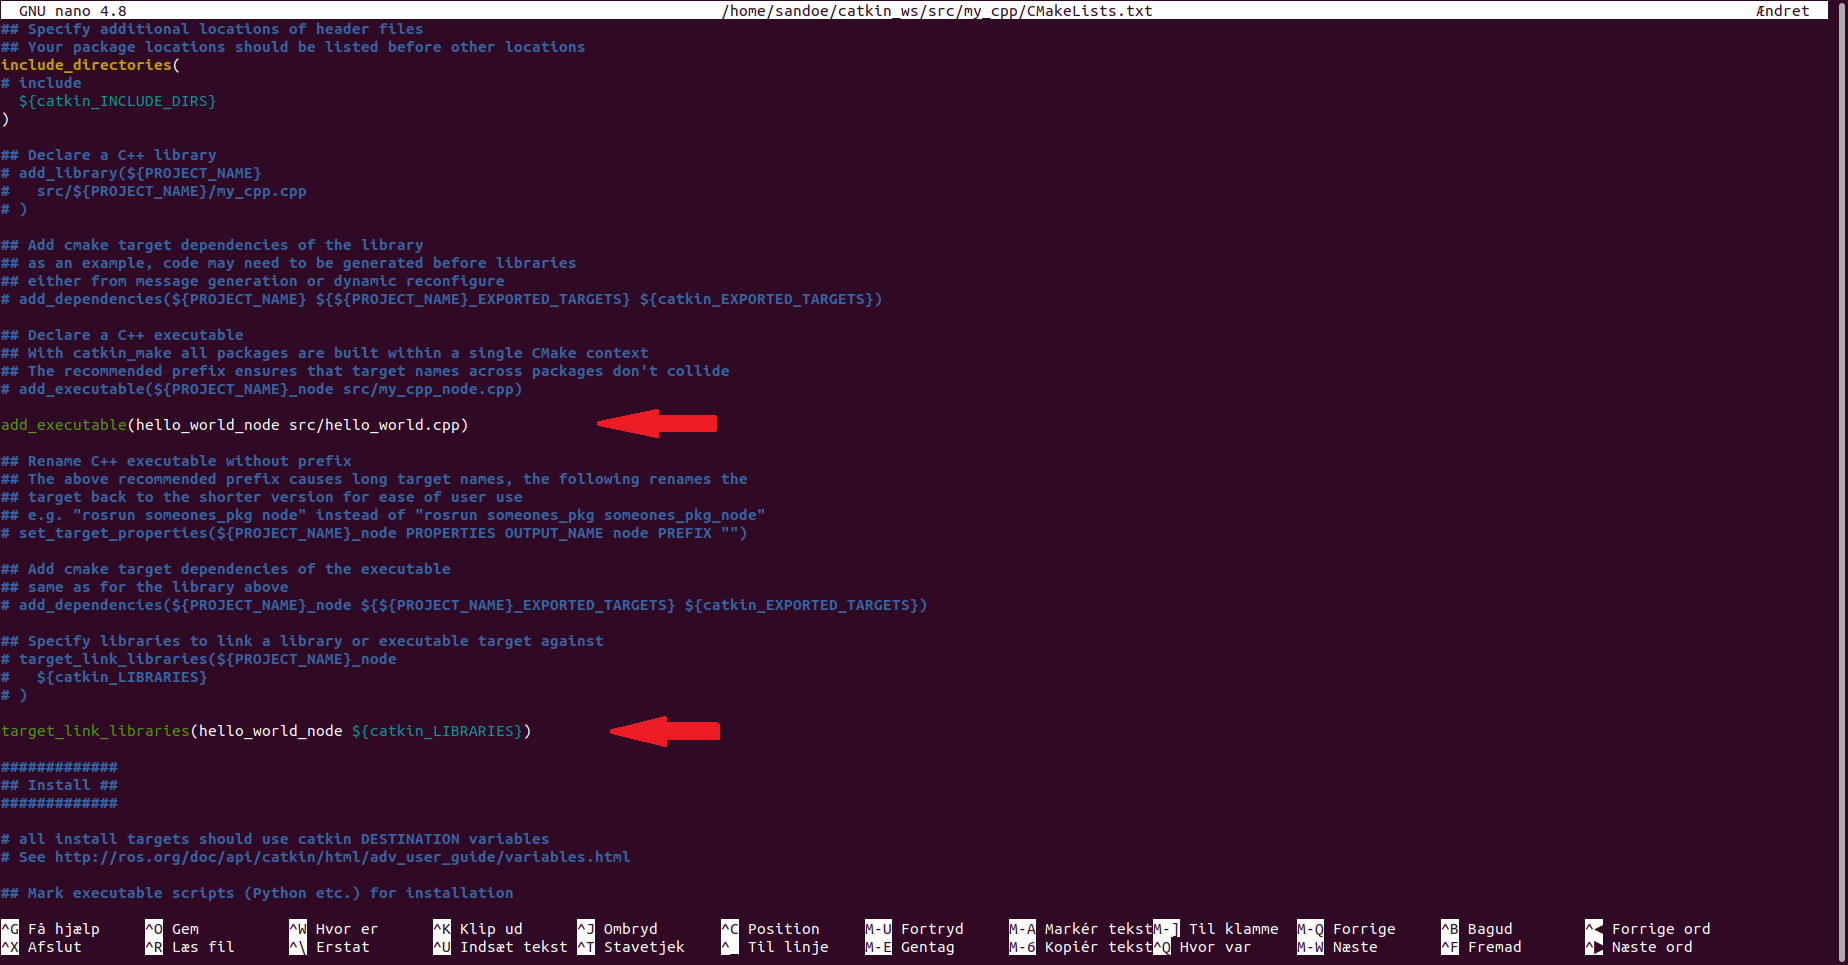
\includegraphics[width=\linewidth]{vmware3}
	\end{figure}
	
	\noindent Build your package again from the workspace root:
	\begin{verbatim}
		cd ~/catkin_ws
		catkin_make
	\end{verbatim}
	
	\section{Run Your ROS Node}
	Make sure ROS master is running by opening a new terminal and typing:
	
	\begin{verbatim}
		roscore
	\end{verbatim}
	In another terminal, run your node:
	
	\begin{verbatim}
		rosrun my_roscpp_package hello_world_node
	\end{verbatim}
	You should now see a "Hello, World from ROS!" message in the terminal.
	
	\section{Source Your Environment (if necessary)}
	If you open a new terminal and ROS cannot find your package or node, you may need to source your workspace's setup script again:
	
	\begin{verbatim}
		source ~/catkin_ws/devel/setup.bash
	\end{verbatim}
	This is the basic process for creating and running a simple ROS node in C++ using roscpp. From here, you can start expanding your node with more functionality, subscribing to topics, publishing messages, and much more.
	
	\section{Installing MATLAB on Ubuntu with Robotics Toolbox}
	\subsection{Introduction}
	This guide will walk you through the process of installing MATLAB on Ubuntu and ensuring that the Robotics Toolbox is included as part of your installation.
	
	\subsection{Step 1: Download MATLAB}
	First, you need to download MATLAB from the official MathWorks website.
	\begin{enumerate}
		\item Visit \url{https://www.mathworks.com/products/matlab.html} and log in with your MathWorks account. If you do not already have an account, you will need to create one.
		\item Once logged in, navigate to the downloads section and select the Linux platform for download.
		\item Download the installer file to your Ubuntu machine.
	\end{enumerate}
	
	\subsection{Step 2: Prepare the Installation}
	After downloading, make the installer executable and run it.
	\begin{verbatim}
	$ cd ~/Downloads
	$ chmod +x matlab_R20XXx_glnxa64.sh
	$ sudo ./matlab_R20XXx_glnxa64.sh
	\end{verbatim}
	Replace \texttt{R20XXx} with the actual version of MATLAB you have downloaded.
	
	\subsection{Step 3: Complete the Installation}
	Follow the on-screen installation guide.
	\begin{enumerate}
		\item When prompted, log in with your MathWorks account.
		\item Accept the license agreement.
		\item Select the installation folder (default is usually fine).
		\item When you reach the step to choose the products you want to install, make sure to \textbf{check Robotics Toolbox}.
		\item Continue through the installation wizard and finish the installation.
	\end{enumerate}
	
	\subsection{Step 4: Activate MATLAB}
	After installation, you need to activate MATLAB with your license. This is usually done at the first startup of MATLAB.
	
	\subsection{Conclusion}
	After these steps, MATLAB should be installed on your Ubuntu machine with the Robotics Toolbox ready for use. For further support, visit the official MathWorks support page.
	
	
\end{document}